\documentclass[a4paper,12pt]{article}
\usepackage[T1]{fontenc}
\usepackage{xcolor}
\usepackage{amssymb,amsmath,bm}
\usepackage[utf8]{inputenc}
\usepackage{amsmath, amssymb, amsfonts}
\usepackage{tikz}
\usetikzlibrary{calc, intersections, through, arrows, backgrounds}
\usetikzlibrary{arrows.meta}

\begin{document}

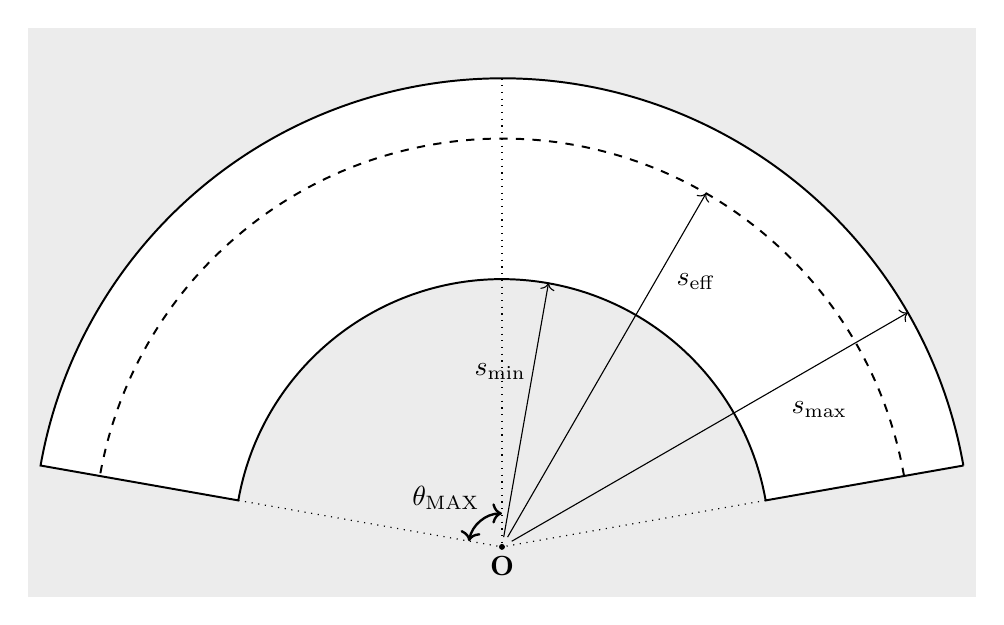
\begin{tikzpicture}[scale=0.85,
    background rectangle/.style={fill=gray!15},
    show background rectangle
                    ]

    \def\Runo{4}
    \def\Rdue{7}
    \def\Reff{6.1}
    \def\s{0.3*\Reff}
    \def\mispunto{1pt}

    \def\thet{80}
    \def\costheta{ 0.17364817766693041 }
    \def\sintheta{ 0.984807753012208 }

    \def\xpuntouno{\Rdue}
    \def\ypuntouno{0.0}
    \node [name=O] at (\xpuntouno,\ypuntouno) {};

    \def\alphadue{30}
    \def\cosalphadue{ 0.8660254037844387 }
    \def\sinalphadue{ 0.5 }
    \def\xpuntodue{\Rdue + \Rdue * \cosalphadue}
    \def\ypuntodue{\Rdue * \sinalphadue}

    \def\alphatre{80}
    \def\cosalphatre{ 0.17364817766693041 }
    \def\sinalphatre{ 0.984807753012208 }
    \def\xpuntotre{\Rdue + \Runo * \cosalphatre}
    \def\ypuntotre{\Runo * \sinalphatre}

    \def\alphaquattro{60}
    \def\cosalphaquattro{ 0.5 }
    \def\sinalphaquattro{ 0.8660254037844387 }
    \def\xpuntoquattro{\Rdue + \Reff * \cosalphaquattro}
    \def\ypuntoquattro{\Reff * \sinalphaquattro}



    \fill [white] (\xpuntouno, \ypuntouno) -- (\xpuntouno + \sintheta * \Rdue, \costheta * \Rdue) arc (90-\thet:90+\thet:\Rdue) -- (\xpuntouno, \ypuntouno);

    \fill [gray!15] (\xpuntouno, \ypuntouno) -- (\xpuntouno +\sintheta * \Runo, \costheta * \Runo) arc (90-\thet:90+\thet:\Runo) -- (\xpuntouno, \ypuntouno);

    \draw [line width=0.25mm] (\xpuntouno + \sintheta * \Rdue, \costheta * \Rdue)
        arc (90-\thet:90+\thet:\Rdue) --
        (\xpuntouno - \sintheta * \Runo, \costheta * \Runo)  --
        (\xpuntouno - \sintheta * \Runo, \costheta * \Runo) arc (90+\thet:90-\thet:\Runo) --
        (\xpuntouno + \sintheta * \Rdue, \costheta * \Rdue);
    \draw [line width=0.25mm, dashed] (\xpuntouno + \sintheta * \Reff, \costheta * \Reff)
        arc (90-\thet:90+\thet:\Reff);

    \draw[line width = 0.15mm, dotted] (\xpuntouno - \sintheta * \Runo, \costheta * \Runo) -- (\xpuntouno, \ypuntouno);
    \draw[line width = 0.15mm, dotted] (\xpuntouno + \sintheta * \Runo, \costheta * \Runo) -- (\xpuntouno, \ypuntouno);
    \draw[line width = 0.15mm, dotted] (\xpuntouno, \Rdue) -- (\xpuntouno, \ypuntouno);

    \def\radcicletheta{0.5}
    \draw[line width = 0.3 mm, <->] (\xpuntouno - \sintheta * \radcicletheta, \costheta * \radcicletheta) arc (90+\thet:90:\radcicletheta);
    \draw[above] node(te) at  (\xpuntouno - 1.7 * \sintheta * \radcicletheta, 4.7*\costheta * \radcicletheta) {$\theta_\mathrm{MAX}$};


    \draw[below] node at (O) {$\mathbf{O}$};
    \filldraw[black, above] (O)circle (\mispunto);


    \draw[->] (O) to (\xpuntodue, \ypuntodue);
    \draw[->] (O) to (\xpuntotre, \ypuntotre);
    \draw[->] (O) to (\xpuntoquattro, \ypuntoquattro);

    \draw[left] node at (\xpuntouno + 0.5, 0.75*\ypuntodue) {$s_\mathrm{min}$};
    \draw[left] node at (\xpuntouno + 5.3, 0.52*\ypuntotre) {$s_\mathrm{max}$};
    \draw[above] node at (\xpuntouno + 2.9, 0.7*\ypuntoquattro) {$s_\mathrm{eff}$};



\end{tikzpicture}

\end{document}